\section{Schéma entité relation}

\section{Schéma logique relationnel}
\subsection{Code DBML}
\inputminted[breaklines =true, autogobble, linenos, frame = single]{sql}{Codes/code_dbml.tex}


\section{PhpMyAdmin}
\subsubsection{Création des foreign keys}
\begin{figure}[H]
    \centering
    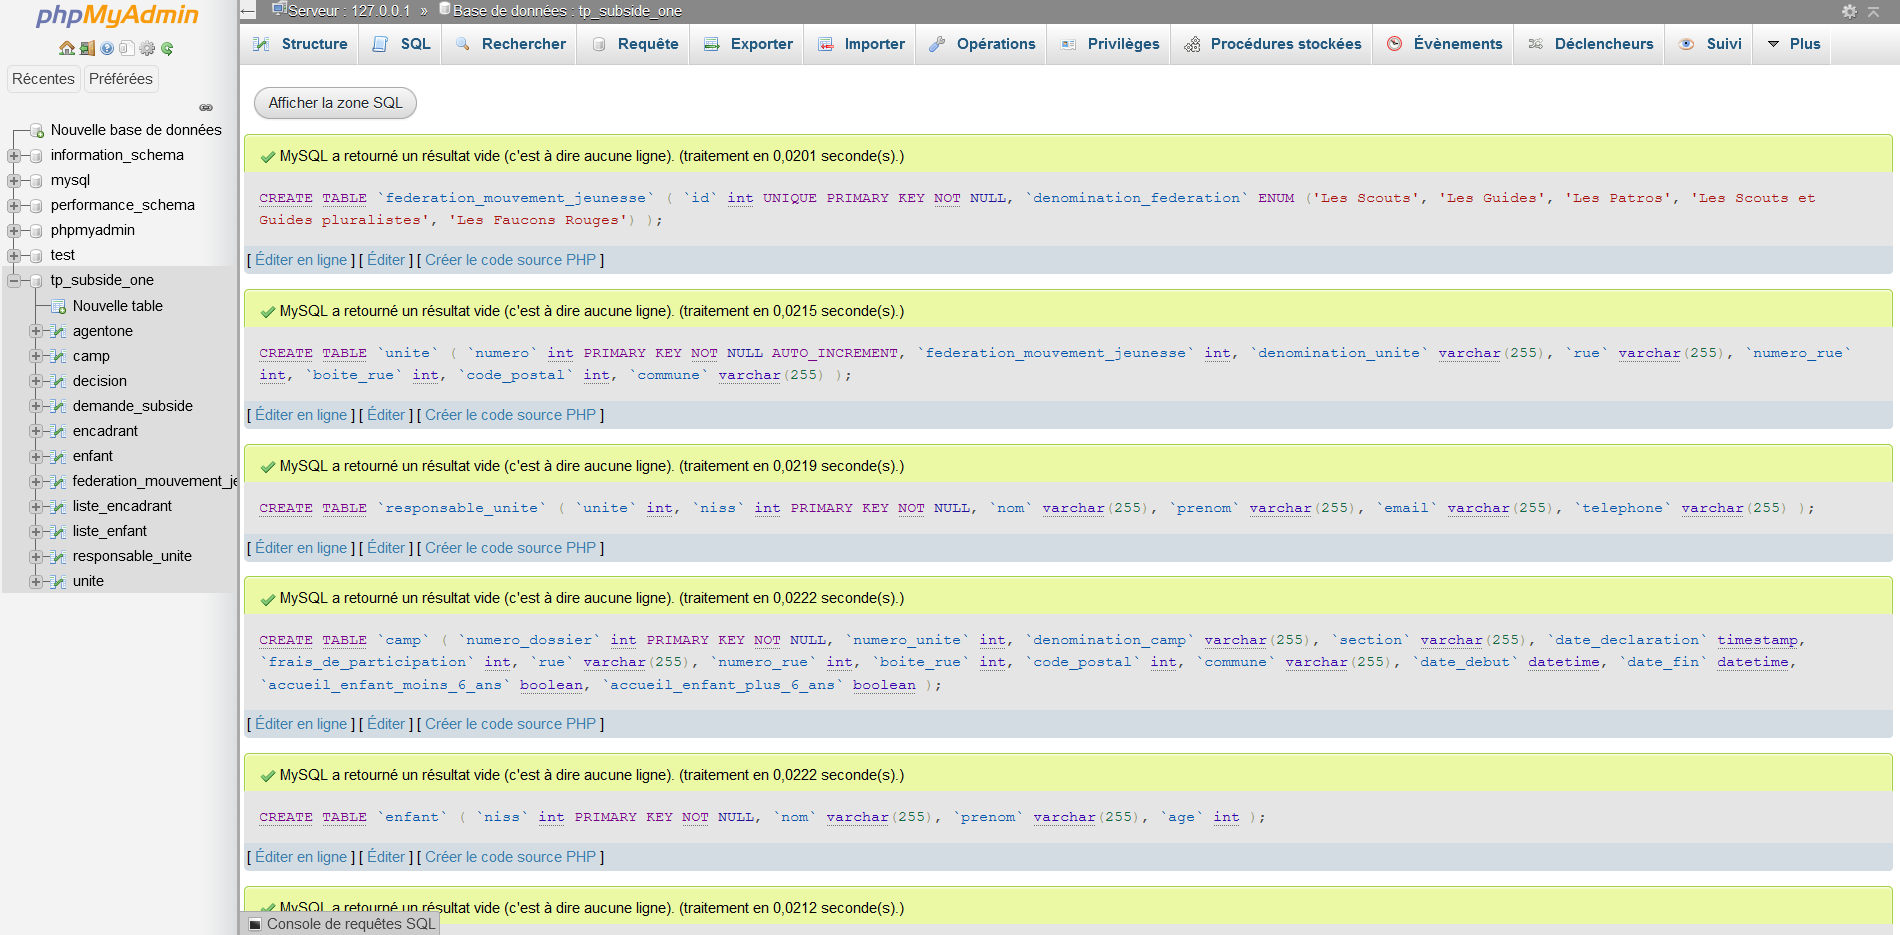
\includegraphics[width=15cm]{Appendix/phpmyadmin_creation_table.png}
    \caption{Caption}
    \label{fig:pmy_creation_fk}
\end{figure}


\section{Script SQL INSERT pour peupler la base de données}

\subsection{Code de création des cinq Mouvements de jeunesse}

Ce code respecte les règles de clé étrangère.
\inputminted[breaklines =true, autogobble, linenos, frame = single]{sql}{Codes/code_insert_fmj.tex}


\subsection{Code d'ajout de quelques unités}
Ce code ne respecte pas les règles de clé étrangère. Il faut désactiver l'option "Activer la vérification des clés étrangères".
\inputminted[breaklines =true, autogobble, linenos, frame = single]{sql}{Codes/code_insert_unite.tex}
